% $Header: /cvsroot/latex-beamer/latex-beamer/examples/beamerexample5.tex,v 1.22 2004/10/08 14:02:33 tantau Exp $

\documentclass[11pt]{beamer}

\usetheme{Darmstadt}

\usepackage{times}
\usefonttheme{structurebold}

%\usepackage[english]{babel}
\usepackage[portuges]{babel}
\usepackage{pgf,pgfarrows,pgfnodes,pgfautomata,pgfheaps}
\usepackage{amsmath,amssymb}
%\usepackage[latin8]{inputenc}
\usepackage[utf8]{inputenc}
\usepackage{graphicx}

\setbeamercovered{dynamic}

\newcommand{\Lang}[1]{\operatorname{\text{\textsc{#1}}}}

\newcommand{\Class}[1]{\operatorname{\mathchoice
  {\text{\sf \small #1}}
  {\text{\sf \small #1}}
  {\text{\sf #1}}
  {\text{\sf #1}}}}

\newcommand{\NumSAT}      {\text{\small\#SAT}}
\newcommand{\NumA}        {\#_{\!A}}

\newcommand{\barA}        {\,\bar{\!A}}

\newcommand{\Nat}{\mathbb{N}}
\newcommand{\Set}[1]{\{#1\}}

\pgfdeclaremask{tu}{beamer-tu-logo-mask}
\pgfdeclaremask{computer}{beamer-computer-mask}
\pgfdeclareimage[interpolate=true,mask=computer,height=2cm]{computerimage}{beamer-computer}
\pgfdeclareimage[interpolate=true,mask=computer,height=2cm]{computerworkingimage}{beamer-computerred}
\pgfdeclareimage[mask=tu,height=.5cm]{logo}{logounesp}

\logo{\pgfuseimage{logo}}

\title{Postulado da Expansão}
\author{Ney Lemke}
\institute[IBB-UNESP]{%
    Mec\^anica Qu\^antica}
\date{2012}                                

\colorlet{redshaded}{red!25!bg}
\colorlet{shaded}{black!25!bg}
\colorlet{shadedshaded}{black!10!bg}
\colorlet{blackshaded}{black!40!bg}

\colorlet{darkred}{red!80!black}
\colorlet{darkblue}{blue!80!black}
\colorlet{darkgreen}{green!80!black}

\def\radius{0.96cm}
\def\innerradius{0.85cm}

\def\softness{0.4}
\definecolor{softred}{rgb}{1,\softness,\softness}
\definecolor{softgreen}{rgb}{\softness,1,\softness}
\definecolor{softblue}{rgb}{\softness,\softness,1}

\definecolor{softrg}{rgb}{1,1,\softness}
\definecolor{softrb}{rgb}{1,\softness,1}
\definecolor{softgb}{rgb}{\softness,1,1}

\newcommand{\Bandshaded}[2]{
  \color{shadedshaded}
  \pgfmoveto{\pgfxy(-0.5,0)}
  \pgflineto{\pgfxy(-0.6,0.1)}
  \pgflineto{\pgfxy(-0.4,0.2)}
  \pgflineto{\pgfxy(-0.6,0.3)}
  \pgflineto{\pgfxy(-0.4,0.4)}
  \pgflineto{\pgfxy(-0.5,0.5)}
  \pgflineto{\pgfxy(4,0.5)}
  \pgflineto{\pgfxy(4.1,0.4)}
  \pgflineto{\pgfxy(3.9,0.3)}
  \pgflineto{\pgfxy(4.1,0.2)}
  \pgflineto{\pgfxy(3.9,0.1)}
  \pgflineto{\pgfxy(4,0)}
  \pgfclosepath
  \pgffill

  \color{black}  
  \pgfputat{\pgfxy(0,0.7)}{\pgfbox[left,base]{#1}}
  \pgfputat{\pgfxy(0,-0.1)}{\pgfbox[left,top]{#2}}
}

\newcommand{\Band}[2]{
  \color{shaded}
  \pgfmoveto{\pgfxy(-0.5,0)}
  \pgflineto{\pgfxy(-0.6,0.1)}
  \pgflineto{\pgfxy(-0.4,0.2)}
  \pgflineto{\pgfxy(-0.6,0.3)}
  \pgflineto{\pgfxy(-0.4,0.4)}
  \pgflineto{\pgfxy(-0.5,0.5)}
  \pgflineto{\pgfxy(4,0.5)}
  \pgflineto{\pgfxy(4.1,0.4)}
  \pgflineto{\pgfxy(3.9,0.3)}
  \pgflineto{\pgfxy(4.1,0.2)}
  \pgflineto{\pgfxy(3.9,0.1)}
  \pgflineto{\pgfxy(4,0)}
  \pgfclosepath
  \pgffill

  \color{black}  
  \pgfputat{\pgfxy(0,0.7)}{\pgfbox[left,base]{#1}}
  \pgfputat{\pgfxy(0,-0.1)}{\pgfbox[left,top]{#2}}
}

\newcommand{\BaenderNormal}
{%
  \pgfsetlinewidth{0.4pt}
  \color{black}
  \pgfputat{\pgfxy(0,5)}{\Band{input tapes}{}}
  \pgfputat{\pgfxy(0.35,4.6)}{\pgfbox[center,base]{$\vdots$}}
  \pgfputat{\pgfxy(0,4)}{\Band{}{}}

  \pgfxyline(0,5)(0,5.5)
  \pgfxyline(1.2,5)(1.2,5.5)
  \pgfputat{\pgfxy(0.25,5.25)}{\pgfbox[left,center]{$w_1$}}

  \pgfxyline(0,4)(0,4.5)
  \pgfxyline(1.8,4)(1.8,4.5)        
  \pgfputat{\pgfxy(0.25,4.25)}{\pgfbox[left,center]{$w_n$}}
  \ignorespaces}

\newcommand{\BaenderZweiNormal}
{%
  \pgfsetlinewidth{0.4pt}
  \color{black}
  \pgfputat{\pgfxy(0,5)}{\Band{Zwei Eingabeb\~AƒÂƒ\~A‚¤nder}{}}
  \pgfputat{\pgfxy(0,4.25)}{\Band{}{}}

  \pgfxyline(0,5)(0,5.5)
  \pgfxyline(1.2,5)(1.2,5.5)
  \pgfputat{\pgfxy(0.25,5.25)}{\pgfbox[left,center]{$u$}}

  \pgfxyline(0,4.25)(0,4.75)
  \pgfxyline(1.8,4.25)(1.8,4.75)        
  \pgfputat{\pgfxy(0.25,4.5)}{\pgfbox[left,center]{$v$}}
  \ignorespaces}

\newcommand{\BaenderHell}
{%
  \pgfsetlinewidth{0.4pt}
  \color{black}
  \pgfputat{\pgfxy(0,5)}{\Bandshaded{input tapes}{}}
  \color{shaded}
  \pgfputat{\pgfxy(0.35,4.6)}{\pgfbox[center,base]{$\vdots$}}
  \pgfputat{\pgfxy(0,4)}{\Bandshaded{}{}}

  \color{blackshaded}
  \pgfxyline(0,5)(0,5.5)
  \pgfxyline(1.2,5)(1.2,5.5)
  \pgfputat{\pgfxy(0.25,5.25)}{\pgfbox[left,center]{$w_1$}}

  \pgfxyline(0,4)(0,4.5)
  \pgfxyline(1.8,4)(1.8,4.5)        
  \pgfputat{\pgfxy(0.25,4.25)}{\pgfbox[left,center]{$w_n$}}
  \ignorespaces}

\newcommand{\BaenderZweiHell}
{%
  \pgfsetlinewidth{0.4pt}
  \color{black}
  \pgfputat{\pgfxy(0,5)}{\Bandshaded{Zwei Eingabeb\~AƒÂƒ\~A‚¤nder}{}}%
  \color{blackshaded}
  \pgfputat{\pgfxy(0,4.25)}{\Bandshaded{}{}}
  \pgfputat{\pgfxy(0.25,4.5)}{\pgfbox[left,center]{$v$}}
  \pgfputat{\pgfxy(0.25,5.25)}{\pgfbox[left,center]{$u$}}%

  \pgfxyline(0,5)(0,5.5)
  \pgfxyline(1.2,5)(1.2,5.5)

  \pgfxyline(0,4.25)(0,4.75)
  \pgfxyline(1.8,4.25)(1.8,4.75)        
  \ignorespaces}

\newcommand{\Slot}[1]{%
  \begin{pgftranslate}{\pgfpoint{#1}{0pt}}%
    \pgfsetlinewidth{0.6pt}%
    \color{structure}%
    \pgfmoveto{\pgfxy(-0.1,5.5)}%
    \pgfbezier{\pgfxy(-0.1,5.55)}{\pgfxy(-0.05,5.6)}{\pgfxy(0,5.6)}%
    \pgfbezier{\pgfxy(0.05,5.6)}{\pgfxy(0.1,5.55)}{\pgfxy(0.1,5.5)}%
    \pgflineto{\pgfxy(0.1,4.0)}%
    \pgfbezier{\pgfxy(0.1,3.95)}{\pgfxy(0.05,3.9)}{\pgfxy(0,3.9)}%
    \pgfbezier{\pgfxy(-0.05,3.9)}{\pgfxy(-0.1,3.95)}{\pgfxy(-0.1,4.0)}%
    \pgfclosepath%
    \pgfstroke%
  \end{pgftranslate}\ignorespaces}

\newcommand{\SlotZwei}[1]{%
  \begin{pgftranslate}{\pgfpoint{#1}{0pt}}%
    \pgfsetlinewidth{0.6pt}%
    \color{structure}%
    \pgfmoveto{\pgfxy(-0.1,5.5)}%
    \pgfbezier{\pgfxy(-0.1,5.55)}{\pgfxy(-0.05,5.6)}{\pgfxy(0,5.6)}%
    \pgfbezier{\pgfxy(0.05,5.6)}{\pgfxy(0.1,5.55)}{\pgfxy(0.1,5.5)}%
    \pgflineto{\pgfxy(0.1,4.25)}%
    \pgfbezier{\pgfxy(0.1,4.25)}{\pgfxy(0.05,4.15)}{\pgfxy(0,4.15)}%
    \pgfbezier{\pgfxy(-0.05,4.15)}{\pgfxy(-0.1,4.2)}{\pgfxy(-0.1,4.25)}%
    \pgfclosepath%
    \pgfstroke%
  \end{pgftranslate}\ignorespaces}

\newcommand{\ClipSlot}[1]{%
  \pgfrect[clip]{\pgfrelative{\pgfxy(-0.1,0)}{\pgfpoint{#1}{4cm}}}{\pgfxy(0.2,1.5)}\ignorespaces}

\newcommand{\ClipSlotZwei}[1]{%
  \pgfrect[clip]{\pgfrelative{\pgfxy(-0.1,0)}{\pgfpoint{#1}{4.25cm}}}{\pgfxy(0.2,1.25)}\ignorespaces}


\AtBeginSection[]{\frame{\frametitle{Outline}\tableofcontents[current]}}

\begin{document}

\frame{\titlepage}

%\section*{Outline}

\frame{\frametitle{Outline}\tableofcontents} 



\section{Autovalores e autofunções}

\frame{\frametitle{Equação de Schrödinger}
$$i\hbar\frac{\partial\psi }{\partial t}=\left[ \frac{-\hbar^2}{2 m}\frac{\partial^2 \psi (x,t)}{\partial x^2} +V(x)\right] \psi(x,t)=\hat{H}\psi(x,t)$$

Separação de Valores:

$$\psi(x,t)=u(x)T(t)$$

Usando separação de variáveis tempos que:

$$\frac{i\hbar T^\prime}{T}=-\frac{\hbar^2}{2m} \frac{u^{\prime\prime}}{u} +V$$

$$i\hbar T^\prime=ET\quad T(t)=Ae^{-i\hbar Et/\hbar}$$

}

\frame{\frametitle{Equação de Autovalores}

$$-\frac{\hbar^2}{2 m}\frac{d^2 u}{dx^2}+V(x)u(x)=Eu(x)$$

$$\hat{H}u=Eu$$

}

\frame{\frametitle{Operador Linear} 
Um operador Linear deve satisfazer asseguintes condições:

\begin{enumerate}
\item $L(\alpha u_1)=\alpha L(u_1)$
\item $L(u_1+u_2)=L(u_1)+L(u_2)$
\item $L(0)=0$
\end{enumerate}


}
\frame{\frametitle{Operadores Lineares - Exemplos}

$$\hat{L}=\frac{df(x)}{dx}-2f(x)$$

$$\hat{p}=-i\hbar \frac{d}{dx}$$

$$\hat{H}=-\frac{\hbar^2}{2m}\frac{d^2}{dx^2}+V(x)$$

}

\frame{\frametitle{Postulado da Expansão}

A função de onda pode ser escrita como:

$$\psi(x,t)=\sum_n C_n u_n(x)e^{-iE_n t/\hbar}+$$
$$\int dEC(E)u_E(x)e^{-iE t/\hbar}$$

}

\section{Partícula em uma Caixa}

\frame{\frametitle{Descrição Física}
\begin{tabular}{c c}
   \begin{minipage}{0.45\textwidth}
 \begin{center}
    \includegraphics[scale=0.3]{infinitewell2.png}
  \end{center}
    \end{minipage}&
    \begin{minipage}{0.45\textwidth} 
  \begin{center}
    \includegraphics[scale=0.3]{infinitewell.png}
  \end{center}
 \end{minipage}
\end{tabular}
}

\frame{\frametitle{Descrição Matemática}

$$u(0)=u(a)=0$$

A equação de Schrödinger nesse caso pode ser escrita como:

$$\frac{d^2 u}{dx^2}+\frac{2m E u}{\hbar^2}=0$$

$$k^2=\frac{2m|E|}{\hbar^2}$$
}


\frame{\frametitle{Autofunções}
  \begin{description}
  \item[$E<0$] 
$$u^{\prime\prime}-k^2u=0\quad u=Ae{\pm k x}$$
Não satisfaz as condições de contorno.
  \item[$E>0$] 
$$u^{\prime\prime}+k^2u=0$$

$$u(x)=A \sin kx + B \cos kx$$

Usando a condição de contorno, temos que $B=0$ e

$$ka=n\pi$$

  \end{description}
}

\frame{\frametitle{Autovalores de Energia}
$$E_n=\frac{\pi^2\hbar^2n^2}{2m  a^2}\quad n=1,2,3,\ldots$$

$$u_n(x)=A\sin\left( \frac{n\pi x}{a}\right)$$

}

\frame{\frametitle{Normalização}

$$\int_0^a \,dx |A_n|^2 \sin^2\left( \frac{n\pi x}{a}\right)=\frac{a}{2}$$

$$A_n=\sqrt{\frac{2}{a}}$$

$$u_n(x)=\sqrt{\frac{2}{a}}\sin\left( \frac{n\pi x}{a}\right)$$

Note que:

$$\int_0^a u_n(x)u_m(x)\,dx=\delta_{nm}$$
}

\frame{\frametitle{Resultados }

Vamos assumir que a partícula está em um dos seus autoestados $u_n$. 
  \begin{description}
  \item[Estado Fundamental] 
$$E_1=\frac{\hbar^2\pi^2}{2 m^2}$$
\item[Valor esperado Momentum]

  \begin{eqnarray*}
\langle p \rangle &=& \int_0^a \,dx u_n^*(x)\left( -i\hbar \frac{d}{dx}\right)u_n(x)    \\
&=& \frac{-2i\hbar}{a}\int_0^a \, \sin\left( \frac{n\pi x}{a}\right) \cos\left( \frac{n\pi x}{a}\right)dx   =0
  \end{eqnarray*}
  \end{description}




}

\frame{\frametitle{Resultados }
  \begin{description}
  \item[Energia Cinética]

$$\langle p^2 \rangle=2mE=\frac{\pi^2\hbar^2 n^2}{a^2}$$
$$K=\frac{\pi^2\hbar^2 n^2}{2 m a^2}$$
\end{description}
}


\frame{\frametitle{Densidades de Probabilidade}

  \begin{center}
    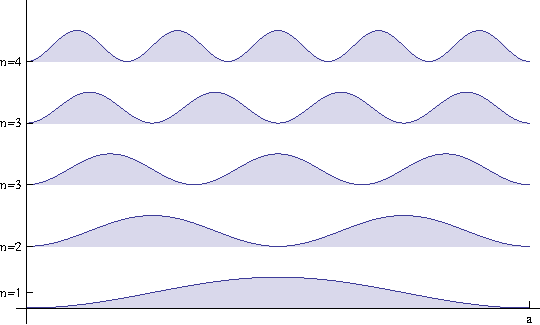
\includegraphics[scale=1.0]{welldensities}
  \end{center}
}

\frame{\frametitle{Exercício}

Resolva a equação de Schrödinger para uma partícula em uma caixa. A partícula está concentrada na metade da caixa em uma região de tamanho $\delta$.
\begin{itemize}
\item Represente a função de onda.
\item Garanta que a função de onda esteja normalizada.
\item Calcule $A_n$.
\item Escreva $\psi(x,t)$
\item Calcule $\langle p \rangle$ em t=0.
\item Calcule $\langle x \rangle$ em t=0.
\item Calcule $\langle E \rangle$.
\end{itemize}
}

\frame{\frametitle{$\langle H \rangle$}
  \begin{eqnarray*}
\langle H \rangle &=& \int_0^a\, dx \psi^*\hat{H}\psi\\    
&=& \int_0^a\, dx \psi^* \hat{H}\sum_nA_n u_n(x) \\
&=& \int_0^a\, dx \psi^* \sum_nE_n A_n u_n(x) \\
&=&  \sum_n E_n A_n \int_0^a\, dx \psi^* u_n \\
&=&  \sum_n E_n A_n A_n^*= \sum_n E_n |A_n|^2 
  \end{eqnarray*}
}

\frame{\frametitle{Interpretação}

$$\langle H \rangle=\sum_n E_nP_n$$

$P_n$ significa a probabilidade de medir $E_n$!
}

\section{Colapso}

\frame{\frametitle{Colapso}

Se medirmos duas vezes a energia de um sistema (ou qualquer outro observável)
os resultados {\bf devem ser iguais}. A única forma de obtermos isso
é que a função de onda colapse após a primeira medida. 
}


\frame{\frametitle{Comentários}
  \begin{itemize}
  \item O colapso ocorre para garantir a objetividade das medidas físicas.
  \item O colapso é um processo não descrito pela eq. de Schrödinger.
  \item O colapso ocorre quando existe interação entre o objeto quantico e 
um objeto macroscópico.
  \end{itemize}
}

\frame{\frametitle{Partícula em um anel}
Considere uma partícula em um anel de raio unitário. 


$$\frac{-\hbar^2}{2m}\frac{d^2u}{dx^2}=Eu\quad \frac{d^2u}{dx^2}+\frac{2 m E}{\hbar^2}u=0$$

$$k^2=\frac{2m E}{\hbar^2} \quad u(0)=u(2\pi)=0$$


$$u_n=A_n e^{ik\varphi}$$

Aplicando a condição de contorno:

$$2k\pi=2n\pi\quad k=n$$

}

 \frame{\frametitle{Partícula em um anel}

 Além dissso as funções devem ser normalizadas:

 $$\int_0^{2\pi} |A_n|^2 u^*_n(x)u_n(x) dx=1\quad A_n=\frac{1}{\sqrt{2\pi}}$$ 

 As funções de onda:


 $$u_n=\frac{1}{\sqrt{2\pi}}e^{in\varphi} \quad n=\ldots,-1,0,1,\ldots$$
 }


\frame{\frametitle{Partícula em um anel-Exercício}
Suponha $\psi(\varphi)=N\cos^2 (\varphi)$

 \begin{itemize}
\item Determne $N$ para que a função esteja normalizada.
  \item Qual é a probabilidade de medirmos $n=-2$?
  \end{itemize}

}

\section{Outros Resultados}
\frame{\frametitle{Autofunção de momento}

Dizemos que um determinado autovalor é degenerado se existirem dois autovetores
ou autofunções diferentes com o mesmo autovalor. 

{\bf Exemplo:}

Considere a partícula livre:

$$\hat{ H}=\frac{\hat{p}^2}{2 m}$$
 
As autofunções:

$$\frac{1}{\sqrt 2\pi \hbar} e^{i k x} \quad 
  \frac{1}{\sqrt 2\pi \hbar} e^{-i k x}$$

Possuem a mesma energia. 
}

\frame{\frametitle{Operador Paridade}

$$P\psi(x)=\psi(-x)$$

$$P u=\lambda u\quad P^2 u=\lambda^2u=u$$

$$\lambda=\pm 1$$

$$P\psi^+(x)=\psi^+(x) \quad P\psi^-(x)=-\psi^-(x)$$

Qualquer função $\psi$ pode ser escrita como a soma de autofunções
do operador paridade.

$$\psi=\frac{1}{2}\left[ \psi(x)+\psi(-x) \right]+
       \frac{1}{2}\left[ \psi(x)-\psi(-x) \right]$$
}

\frame{\frametitle{Operador Paridade}
Considere:

$$\psi(x,0)=\psi(-x,0)=\psi^+(x)$$

$$i\hbar\frac{\partial \psi}{\partial t}=\hat{H}\psi$$

Vamos assumir que $[\hat{P},\hat{H}]=0$

$$i\hbar\frac{\partial P\psi}{\partial t}=P\hat{H}\psi$$

$$i\hbar\frac{\partial (P\psi)}{\partial t}=\hat{H}(P\psi )$$
}

\frame{\frametitle{Operador Paridade}
Ou seja se $P$ e $H$ comutam se em $t=0$ a função é par 
ela seguirá sendo par em todos os instantes de tempo. Isso ocorre se 
$V(x)=V(-x)$. 

Este resultado é mais geral, seja um operaor $\hat{M}$ e $[\hat{M},\hat{H}]=0$.
Se o sistema inicialmente está em um dos autoestados de $M$ seguirá 
sendo uma autofunção de $\hat{M}$. Nestes casos em analogia 
com a Mecânica Clássica, $M$ é dito uma constante de movimento. 

}
\end{document}
